\chapter{Cristalografia e difração de raios X}\label{ch:b3:x-ray-diffraction}

Em 1912, um feixe de raios X enviado através de um cristal de sulfato de
cobre deixou em uma chapa fotográfica um padrão de manchas nítidas: os
cristais difratam os raios X como uma rede difrata a luz, porque as distâncias
entre seus átomos são comparáveis ao comprimento de onda dos raios X. Um ano
depois, William Lawrence Bragg, então estudante, leu nesses padrões a
estrutura do sal-gema --- e mostrou que o sólido não contém nenhuma molécula de
\ce{NaCl}, apenas uma rede em que cada íon tem seis vizinhos do outro tipo.
Todas as estruturas cristalinas citadas no volume do 1.º ano e neste livro
foram encontradas assim. Este capítulo dá a geometria das redes e de sua
simetria, a condição de difração, as intensidades que revelam o conteúdo da
célula e os métodos de pó e de monocristal usados em todo laboratório.

\begin{recall}
O volume do 1.º ano descreveu os cristais por uma rede de nós, um motivo e uma
célula unitária com seus parâmetros de rede; contou a multiplicidade de uma
célula; construiu as estruturas cúbica de faces centradas, cúbica de corpo
centrado e hexagonal compacta e os tipos sal-gema, cloreto de césio, blenda e
fluorita; e calculou uma densidade a partir de uma célula. O
\cref{ch:b3:point-groups} definiu \omterm{def:b3:point-groups:operation}{operações de simetria} e \omterm{def:b3:point-groups:point-group}{grupos pontuais}.
\end{recall}

\begin{omfigure}
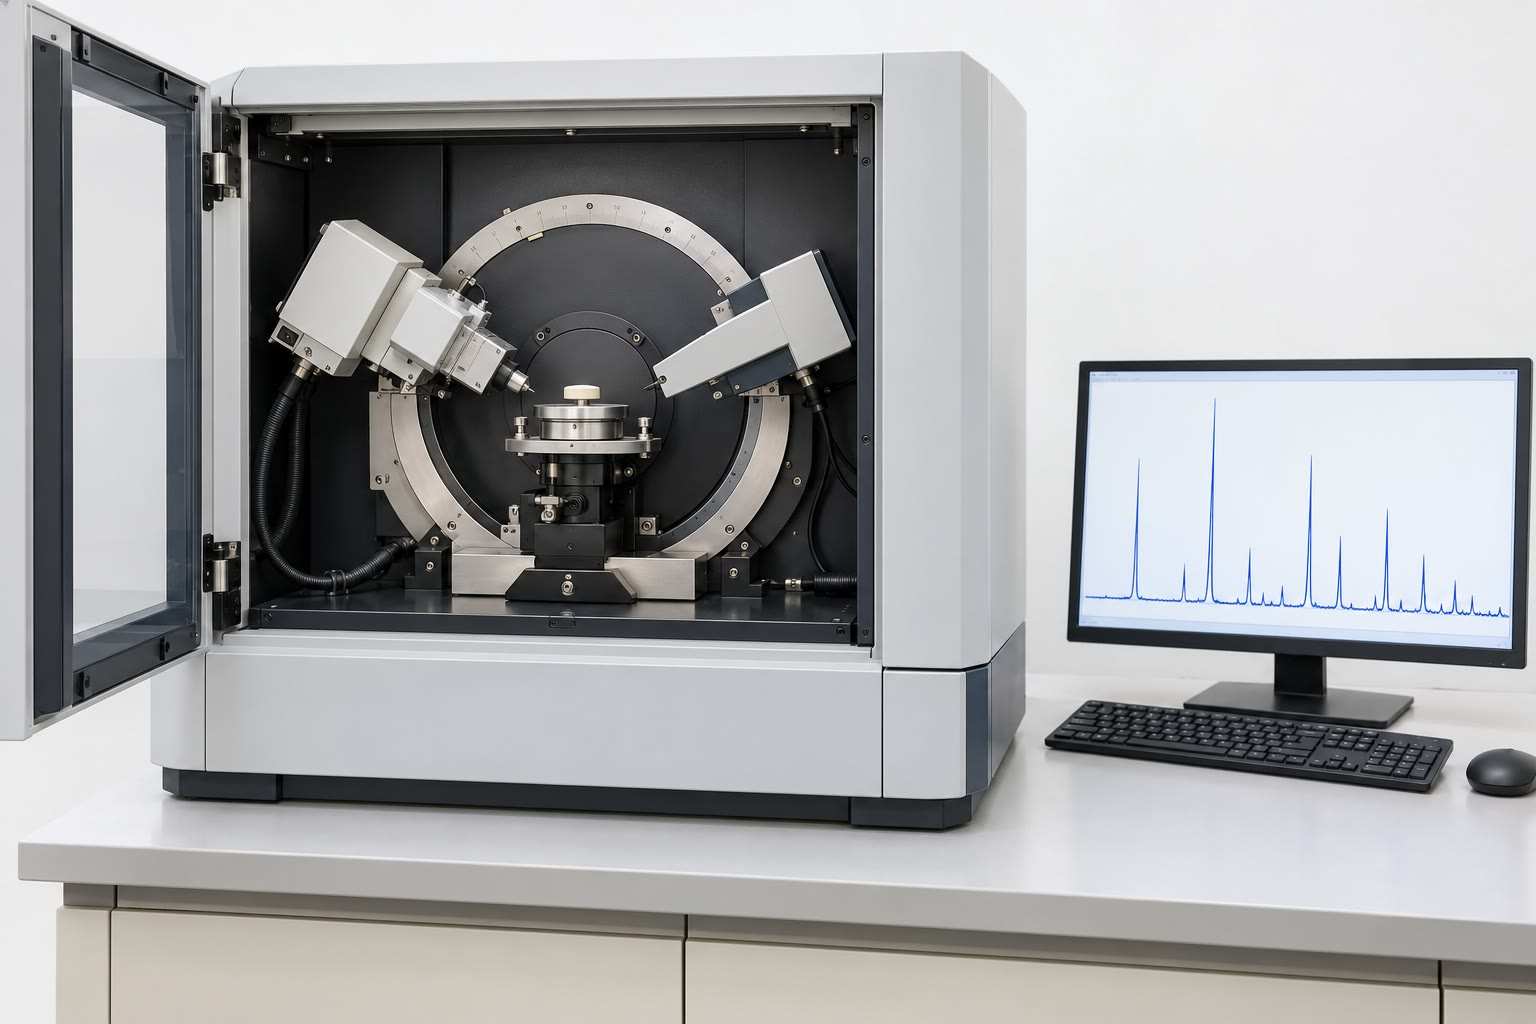
\includegraphics[width=0.6\linewidth]{images/book4/ai/b3-09-diffractometer.jpg}

{\small Um difratômetro de pó de bancada: o tubo de raios X e o detector giram
sobre um círculo em torno da amostra plana.}
\end{omfigure}

\section{Sistemas cristalinos e redes de Bravais}

Uma rede só pode ter \omterm{def:b3:point-groups:operation}{operações de simetria} que a levem sobre si mesma. Isso as
restringe fortemente.

\begin{theorem}[A restrição cristalográfica]\label{thm:b3:x-ray-diffraction:restriction}
Os únicos eixos de rotação compatíveis com uma rede são de ordem 1, 2, 3, 4 e 6.
\end{theorem}

\begin{proof}
Em uma base de vetores da rede, uma rotação de simetria leva vetores da rede em
vetores da rede, logo sua matriz tem entradas inteiras e traço inteiro. O
traço não depende da base; em uma base ortonormal com $z$ ao longo do eixo,
ele vale $1 + 2\cos\theta$. Logo $2\cos\theta$ é um inteiro entre $-2$ e 2:
$\cos\theta \in \{-1, -\frac12, 0, \frac12, 1\}$, $\theta = 180^\circ, 120^\circ, 90^\circ,
60^\circ, 0^\circ$: ordens 2, 3, 4, 6, 1. Um eixo de ordem cinco é impossível.
\end{proof}

\begin{definition}[Sistema cristalino, rede de Bravais, centragem da rede]\label{def:b3:x-ray-diffraction:crystal-system}
As redes são agrupadas por sua simetria em sete \emph{sistemas
cristalinos}\index{sistema cristalino} (triclínico, monoclínico, ortorrômbico, tetragonal,
trigonal, hexagonal, cúbico). Uma célula pode ter nós da rede apenas em seus
vértices (primitiva, P) ou também em seu centro (de corpo centrado, I), nos
centros de todas as faces (de faces centradas, F) ou de um par de faces (de
bases centradas, C), ou ao longo de uma diagonal do corpo (romboédrica, R): é sua
\emph{centragem da rede}\index{centragem da rede}. As 14 combinações distintas de um
sistema e de uma centragem são as \emph{redes de Bravais}\index{rede de Bravais}.
\end{definition}

\begin{center}\small
\begin{tabular}{lll}
\hline
sistema & restrições da célula & centragens \\ \hline
triclínico & nenhuma & P \\
monoclínico & $\alpha = \gamma = 90^\circ$ & P, C \\
ortorrômbico & $\alpha = \beta = \gamma = 90^\circ$ & P, C, I, F \\
tetragonal & $a = b$, todos os ângulos $90^\circ$ & P, I \\
trigonal & $a = b = c$, $\alpha = \beta = \gamma \ne 90^\circ$ (eixos romboédricos) & R \\
hexagonal & $a = b$, $\alpha = \beta = 90^\circ$, $\gamma = 120^\circ$ & P \\
cúbico & $a = b = c$, todos os ângulos $90^\circ$ & P, I, F \\ \hline
\end{tabular}
\end{center}

\begin{omfigure}
\tdplotsetmaincoords{60}{100}
\begin{tikzpicture}[tdplot_main_coords, scale=1.25, font=\small]
  \foreach \s/\lab in {0/{cúbica P}, 3.0/{cúbica I}, 6.0/{cúbica F}}{
    \begin{scope}[xshift=\s cm]
      \pic[transform shape] {omcubeo={1.6}};
      \foreach \x in {0,1.6}{\foreach \y in {0,1.6}{\foreach \z in {0,1.6}{\node[cellA=2.6mm] at (\x,\y,\z) {};}}}
      \node[anchor=north] at (0.8,0.8,-0.62) {\lab};
    \end{scope}}
  \begin{scope}[xshift=3.0cm]
    \node[cellB=2.6mm] at (0.8,0.8,0.8) {};
  \end{scope}
  \begin{scope}[xshift=6.0cm]
    \foreach \p in {(0.8,0.8,0),(0.8,0.8,1.6),(0.8,0,0.8),(0.8,1.6,0.8),(0,0.8,0.8),(1.6,0.8,0.8)}{\node[cellB=2.6mm] at \p {};}
  \end{scope}
\end{tikzpicture}

{\small As três \omterm{def:b3:x-ray-diffraction:crystal-system}{redes de Bravais} cúbicas: primitiva (nós nos vértices), de corpo
centrado (mais o centro, em vermelho) e de faces centradas (mais os seis
centros de faces, em vermelho). Suas células contêm 1, 2 e 4 nós.}
\end{omfigure}

\section{Planos reticulares e a rede recíproca}

\begin{definition}[Plano reticular, índices de Miller, distância interplanar]\label{def:b3:x-ray-diffraction:miller}
Um \emph{plano reticular}\index{plano reticular} é um plano que passa por pelo menos
três nós não alinhados; ele pertence a uma família de planos paralelos e
igualmente espaçados que contém todos os nós. Se o plano da família mais
próximo da origem corta os eixos em $a/h$, $b/k$, $c/l$, os inteiros $(hkl)$, sem
fator comum, são seus \emph{índices de Miller}\index{indices de Miller@índices de Miller} (um índice 0
para um plano paralelo a um eixo). A distância entre planos adjacentes é a
\emph{distância interplanar}\index{distancia interplanar@distância interplanar} $d_{hkl}$.
\end{definition}

\begin{proposition}[Distâncias em células ortogonais]\label{prop:b3:x-ray-diffraction:spacing}
Para uma célula ortorrômbica, $\dfrac{1}{d_{hkl}^2} = \dfrac{h^2}{a^2} + \dfrac{k^2}{b^2} +
\dfrac{l^2}{c^2}$; para uma célula cúbica, $d_{hkl} = a/\sqrt{h^2 + k^2 + l^2}$.
\end{proposition}

\begin{proof}
O plano $hx/a + ky/b + lz/c = 1$ tem vetor normal $\mathbf n = (h/a, k/b, l/c)$
e fica à distância $1/|\mathbf n|$ da origem; o plano paralelo que passa pela
origem pertence à família, logo $d = 1/|\mathbf n|$.
\end{proof}

\begin{definition}[Rede recíproca]\label{def:b3:x-ray-diffraction:reciprocal}
Para uma rede de vetores de base $\mathbf a$, $\mathbf b$, $\mathbf c$ e volume de célula $V$,
a \emph{rede recíproca}\index{rede reciproca@rede recíproca} tem vetores de base
$\mathbf a^* = (\mathbf b\times\mathbf c)/V$, $\mathbf b^* = (\mathbf c\times\mathbf a)/V$,
$\mathbf c^* = (\mathbf a\times\mathbf b)/V$, de modo que $\mathbf a\cdot\mathbf a^* = 1$ e
$\mathbf a\cdot\mathbf b^* = 0$. Seu nó $\mathbf G_{hkl} = h\mathbf a^* + k\mathbf b^* + l\mathbf c^*$ é
perpendicular aos planos $(hkl)$, e $|\mathbf G_{hkl}| = 1/d_{hkl}$.
\end{definition}

\section{Difração}

\begin{theorem}[Lei de Bragg]\label{thm:b3:x-ray-diffraction:bragg}
Raios X de comprimento de onda $\lambda$ são refletidos por uma família de planos de
espaçamento $d$ apenas nos ângulos rasantes $\theta$ que satisfazem
\[
2d\sin\theta = n\lambda, \qquad n = 1, 2, \dots,
\]
a \emph{lei de Bragg}\index{lei de Bragg}. A ordem $n$ é absorvida escrevendo a
reflexão $(nh\,nk\,nl)$ com espaçamento $d/n$.
\end{theorem}

\begin{proof}
Os raios espalhados por dois planos adjacentes, com ângulos iguais de incidência
e de reflexão $\theta$, diferem em caminho de $2d\sin\theta$ (os dois segmentos de cada lado
da normal que passa pelo plano inferior). Eles se reforçam quando essa diferença
é um número inteiro de comprimentos de onda; com milhões de planos, qualquer outro
ângulo dá raios que se cancelam aos pares.
\end{proof}

\begin{omfigure}
\begin{tikzpicture}[font=\small, >=Stealth]
  \foreach \y in {0,-1.1}{\draw[thick] (-0.4,\y) -- (7.4,\y);}
  \foreach \x in {0,1.4,...,7.0}{\fill (\x,0) circle (1.5pt) (\x,-1.1) circle (1.5pt);}
  \draw[->, omDef, thick] (0.2,1.75) -- (2.8,0);
  \draw[->, omDef, thick] (2.8,0) -- (5.4,1.75);
  \draw[->, omDef, thick] (-1.43,1.75) -- (2.8,-1.1);
  \draw[->, omDef, thick] (2.8,-1.1) -- (7.03,1.75);
  \draw[densely dashed] (2.8,0) -- (2.8,-1.1);
  \draw[omThm, thick] (2.8,0) -- (2.18,-0.68) (2.8,0) -- (3.42,-0.68);
  \draw[omThm, very thick] (2.18,-0.68) -- (2.8,-1.1) -- (3.42,-0.68);
  \draw (1.8,0) arc[start angle=180, end angle=213.9, radius=1.0];
  \node[anchor=east] at (1.85,-0.2) {$\theta$};
  \draw[<->] (7.7,0) -- (7.7,-1.1) node[midway, right] {$d$};
  \node[omThm, anchor=north] at (2.8,-1.2) {diferença de caminho $2d\sin\theta$};
\end{tikzpicture}

{\small A construção de Bragg. Os raios refletidos por planos adjacentes
percorrem a mais os dois segmentos vermelhos, de $d\sin\theta$ cada; as ondas se
reforçam quando $2d\sin\theta$ é um número inteiro de comprimentos de onda.}
\end{omfigure}

\begin{proposition}[Condição de Laue]\label{prop:b3:x-ray-diffraction:laue}
Com vetores de onda incidente e espalhado $\mathbf k$ e $\mathbf k'$ de comprimento
$1/\lambda$, há difração quando $\mathbf k' - \mathbf k = \mathbf G_{hkl}$, um vetor da \omterm{def:b3:x-ray-diffraction:reciprocal}{rede
recíproca}; isso é equivalente à \omterm{thm:b3:x-ray-diffraction:bragg}{lei de Bragg}.
\end{proposition}

\begin{proof}
As ondas espalhadas por dois nós separados por um vetor da rede $\mathbf R$ diferem em fase
de $2\pi(\mathbf k' - \mathbf k)\cdot\mathbf R$; todas se reforçam se isso for um múltiplo de $2\pi$
para todo $\mathbf R$, isto é, se $\mathbf k' - \mathbf k$ estiver na \omterm{def:b3:x-ray-diffraction:reciprocal}{rede recíproca} (pela
definição $\mathbf a\cdot\mathbf a^* = 1$, $\mathbf a\cdot\mathbf b^* = 0$\dots). Para o espalhamento elástico,
$|\mathbf k| = |\mathbf k'|$ e $|\mathbf k' - \mathbf k| = 2\sin\theta/\lambda$, onde $2\theta$ é o ângulo
entre eles; com $|\mathbf G| = 1/d$, isso dá $2d\sin\theta = \lambda$, e $\mathbf G$ é normal aos
planos refletores.
\end{proof}

\begin{definition}[Esfera de Ewald]\label{def:b3:x-ray-diffraction:ewald}
A \emph{esfera de Ewald}\index{esfera de Ewald} tem raio $1/\lambda$ e passa pela
origem da \omterm{def:b3:x-ray-diffraction:reciprocal}{rede recíproca}, com centro em $-\mathbf k$ a partir da origem; há uma
reflexão sempre que um nó da \omterm{def:b3:x-ray-diffraction:reciprocal}{rede recíproca} está sobre ela.
\end{definition}

\begin{omfigure}
\begin{tikzpicture}[font=\small, >=Stealth, scale=0.9]
  \foreach \i in {-2,...,4}{\foreach \j in {-2,...,2}{\fill[black!60] (\i*1.0,\j*0.75) circle (1.3pt);}}
  \node[anchor=north east] at (0,0) {$O$};
  \draw[omDef] (-1.625,0.0) circle (1.625);
  \draw[->, omDef, thick] (-1.625,0) -- (0,0) node[midway, below] {$\mathbf k$};
  \draw[->, omThm, thick] (-1.625,0) -- (-1.0,1.5);
  \node[omThm, anchor=east] at (-1.4,0.85) {$\mathbf k'$};
  \draw[->, black, very thick] (0,0) -- (-1.0,1.5) node[pos=0.3, left] {$\mathbf G$};
  \node[anchor=north] at (-1.625,-1.75) {esfera de Ewald, raio $1/\lambda$};
  \draw[<->] (4.6,0) -- (4.6,0.75) node[midway, right] {$b^*$};
  \draw[<->] (3,-1.85) -- (4,-1.85) node[midway, below] {$a^*$};
\end{tikzpicture}

{\small A construção de Ewald em duas dimensões (o círculo passa pela origem
$O$ da \omterm{def:b3:x-ray-diffraction:reciprocal}{rede recíproca}). Um nó $\mathbf G$ sobre o círculo dá um feixe
difratado $\mathbf k' = \mathbf k + \mathbf G$. Aqui o círculo, de raio escolhido para o
desenho, passa pelo nó $(-1, 2)$.}
\end{omfigure}

\section{Intensidades e simetria}

A \omterm{thm:b3:x-ray-diffraction:bragg}{lei de Bragg} dá as direções dos feixes difratados, que dependem apenas da
rede; suas intensidades dependem do que há na célula.

\begin{definition}[Fator de espalhamento atômico, fator de estrutura]\label{def:b3:x-ray-diffraction:structure-factor}
O \emph{fator de espalhamento atômico}\index{fator de espalhamento atomico@fator de espalhamento atômico} $f_j$ de um
átomo é a amplitude que ele espalha, em unidades da de um elétron; ele é igual
a seu número de elétrons na direção dianteira e decresce em ângulos maiores. O
\emph{fator de estrutura}\index{fator de estrutura} da reflexão $hkl$ é
\[
F_{hkl} = \sum_jf_j\,\eu^{2\pi\iu(hx_j + ky_j + lz_j)},
\]
somado sobre os átomos da célula de coordenadas fracionárias $(x_j, y_j, z_j)$.
\end{definition}

\begin{proposition}[Intensidade]\label{prop:b3:x-ray-diffraction:intensity}
A intensidade de uma reflexão é proporcional a $|F_{hkl}|^2$.
\end{proposition}

\begin{proof}[Demonstração parcial]
O átomo $j$ está em $\mathbf r_j = x_j\mathbf a + y_j\mathbf b + z_j\mathbf c$; para uma reflexão,
$(\mathbf k' - \mathbf k)\cdot\mathbf r_j = hx_j + ky_j + lz_j$, logo sua onda tem a fase
$2\pi(hx_j + ky_j + lz_j)$ em relação a um átomo na origem, e amplitude $f_j$:
a célula espalha a soma $F_{hkl}$, e todas as células o mesmo. Uma intensidade é o
quadrado do módulo de uma amplitude. Que o espalhamento múltiplo possa ser
desprezado (a aproximação cinemática) é admitido.
\end{proof}

\begin{definition}[Ausência sistemática]\label{def:b3:x-ray-diffraction:absence}
Uma \emph{ausência sistemática}\index{ausencia sistematica@ausência sistemática} é uma reflexão cujo
\omterm{def:b3:x-ray-diffraction:structure-factor}{fator de estrutura} se anula para todo cristal de uma dada \omterm{def:b3:x-ray-diffraction:crystal-system}{centragem da rede} ou
simetria, quaisquer que sejam seus átomos.
\end{definition}

\begin{proposition}[Ausências das redes centradas]\label{prop:b3:x-ray-diffraction:absences}
Em uma rede de corpo centrado, as reflexões com $h + k + l$ ímpar estão ausentes; em
uma rede de faces centradas, as reflexões com $h$, $k$, $l$ de paridades mistas estão ausentes.
\end{proposition}

\begin{proof}
Centragem I: todo átomo em $(x,y,z)$ tem uma cópia em $(x + \frac12, y + \frac12, z + \frac12)$,
cujo fator de fase difere de $\eu^{\iu\pi(h+k+l)} = (-1)^{h+k+l}$: $F = (1 +
(-1)^{h+k+l})F'$. Centragem F: as cópias em três centros de faces dão o fator $1 +
(-1)^{h+k} + (-1)^{h+l} + (-1)^{k+l}$, igual a 4 se $h$, $k$, $l$ são todos pares ou todos
ímpares, e a 0 caso contrário.
\end{proof}

\begin{example}[Sal-gema e silvita]\label{ex:b3:x-ray-diffraction:nacl-kcl}
% ledger: lat:NaCl, lat:KCl
Na estrutura sal-gema, com os cátions em $(0,0,0)$ e os ânions em $(\frac12,0,0)$, cada um
com as translações F: $F_{hkl} = 4[f_+ + f_-(-1)^{h+k+l}]$ para índices não mistos.
Para \ce{NaCl}, $f(\ce{Na+}) \approx 10$ e $f(\ce{Cl-}) \approx 18$: as reflexões todas ímpares
(111), (311) são fracas, mas presentes. Para \ce{KCl}, \ce{K+} e \ce{Cl-} têm ambos 18
elétrons: as reflexões todas ímpares quase desaparecem, e o difratograma parece
o de uma rede cúbica primitiva com metade da aresta da célula (figura abaixo).
\end{example}

\begin{omfigure}
\begin{tikzpicture}
\begin{axis}[name=salts, width=0.95\linewidth, height=5.2cm, xmin=20, xmax=90,
  ymin=0, ymax=2.55, ytick=\empty, axis x line=bottom, axis y line=none,
  xlabel={$2\theta$ / grau (Cu K$\alpha_1$)}, tick label style={font=\small},
  label style={font=\small}]
\addplot[omDef, thin] table[x=tt, y expr=\thisrow{NaCl}+1.35] {figdata/out/bachelor-3-xrd-powder-salts.dat};
\addplot[omThm, thin] table[x=tt, y=KCl] {figdata/out/bachelor-3-xrd-powder-salts.dat};
\node[font=\small, omDef, anchor=west] at (axis cs:79,1.9) {\ce{NaCl}};
\node[font=\small, omThm, anchor=west] at (axis cs:77,0.55) {\ce{KCl}};
\node[font=\scriptsize, anchor=south] at (axis cs:27.36,1.52) {111};
\node[font=\scriptsize, anchor=west] at (axis cs:32.1,2.25) {200};
\node[font=\scriptsize, anchor=west] at (axis cs:28.8,0.9) {200};
\node[font=\scriptsize, anchor=west] at (axis cs:41.0,0.85) {220};
\end{axis}
\end{tikzpicture}

\begin{tikzpicture}
\begin{axis}[name=met, width=0.62\linewidth, height=4.4cm, xmin=35, xmax=100,
  ymin=0, ymax=2.35, ytick=\empty, axis x line=bottom, axis y line=none,
  xlabel={$2\theta$ / grau}, tick label style={font=\small}, label style={font=\small}]
\addplot[omDef, thin] table[x=tt, y expr=\thisrow{Cu}+1.2] {figdata/out/bachelor-3-xrd-powder-metals.dat};
\addplot[omThm, thin] table[x=tt, y=W] {figdata/out/bachelor-3-xrd-powder-metals.dat};
\node[font=\small, omDef, anchor=west] at (axis cs:55,1.5) {Cu (F)};
\node[font=\small, omThm, anchor=west] at (axis cs:44,0.4) {W (I)};
\end{axis}
\begin{axis}[at={(met.east)}, anchor=west, xshift=0.7cm, width=0.36\linewidth, height=4.4cm,
  xmin=29.7, xmax=33.7, ymin=0, ymax=1.1, ytick=\empty, axis x line=bottom,
  axis y line=none, xlabel={$2\theta$ / grau}, tick label style={font=\small},
  label style={font=\small}, title={\small Scherrer}]
\addplot[black, thick] table[x=tt, y=L200] {figdata/out/bachelor-3-xrd-powder-scherrer.dat};
\addplot[omDef, thick] table[x=tt, y=L50] {figdata/out/bachelor-3-xrd-powder-scherrer.dat};
\addplot[omThm, thick] table[x=tt, y=L10] {figdata/out/bachelor-3-xrd-powder-scherrer.dat};
\end{axis}
\end{tikzpicture}

{\small \omterm{def:b3:x-ray-diffraction:powder}{Difratogramas de pó} calculados (Cu K$\alpha_1$; fatores de espalhamento tomados
iguais aos números de elétrons, de modo que só as ausências e as tendências gerais
de intensidade têm significado). Em cima: \ce{NaCl} e \ce{KCl}; as linhas todas
ímpares de \ce{KCl} desaparecem. Embaixo, à esquerda: o cobre (F) mostra (111), (200),
(220), (311)\dots; o tungstênio (I) mostra (110), (200), (211)\dots. Embaixo, à
direita: a linha (200) de \ce{NaCl} para cristalitos de 200 (preto), 50 (azul) e
10 nm (vermelho): cristais menores dão linhas mais largas.}
\end{omfigure}

\begin{proposition}[Lei de Friedel]\label{prop:b3:x-ray-diffraction:friedel}
Na ausência de espalhamento anômalo, $|F_{hkl}| = |F_{\bar h\bar k\bar l}|$: um difratograma
parece centrossimétrico mesmo quando o cristal não é.
\end{proposition}

\begin{proof}
Com $f_j$ reais, $F_{\bar h\bar k\bar l} = \sum f_j\eu^{-2\pi\iu(\dots)} = F_{hkl}^*$, de mesmo
módulo.
\end{proof}

\omterm{def:b3:point-groups:operation}{Elementos de simetria} que combinam uma rotação ou uma reflexão com uma fração de
uma translação da rede só existem nos cristais.

\begin{definition}[Eixo helicoidal, plano de deslizamento, grupo espacial]\label{def:b3:x-ray-diffraction:space-group}
Um \emph{eixo helicoidal}\index{eixo helicoidal} $n_p$ combina uma rotação de $2\pi/n$ com
uma translação de $p/n$ do período da rede ao longo do eixo ($2_1$: meia volta e
meia célula). Um \emph{plano de deslizamento}\index{plano de deslizamento} combina uma
reflexão com uma translação de meio vetor da rede paralela ao plano
(deslizamentos $a$, $b$, $c$). O grupo de todas as \omterm{def:b3:point-groups:operation}{operações de simetria} de um cristal,
translações incluídas, é seu \emph{grupo espacial}\index{grupo espacial}: há 230. A
menor parte dele a partir da qual as operações geram todo o cristal é a
\emph{unidade assimétrica}\index{unidade assimetrica@unidade assimétrica}. Um conjunto de pontos
deixados em si mesmos por um \omterm{def:b3:point-groups:class}{subgrupo} das operações é uma \emph{posição de
Wyckoff}\index{posicao de Wyckoff@posição de Wyckoff}: as posições gerais não têm simetria, as posições
especiais ficam sobre \omterm{def:b3:point-groups:operation}{elementos de simetria}.
\end{definition}

\begin{proposition}[Ausências devidas a um eixo helicoidal]\label{prop:b3:x-ray-diffraction:screw-absence}
Um eixo $2_1$ ao longo de $b$ torna ausentes as reflexões $0k0$ com $k$ ímpar.
\end{proposition}

\begin{proof}
O eixo leva $(x, y, z)$ a $(-x, y + \frac12, -z)$. Para $h = l = 0$, os dois átomos têm
os fatores de fase $\eu^{2\pi\iu ky}$ e $\eu^{2\pi\iu k(y + 1/2)} = (-1)^k\eu^{2\pi\iu ky}$: sua soma
se anula para $k$ ímpar.
\end{proof}

\begin{method}[Ler o símbolo de um grupo espacial]\label{met:b3:x-ray-diffraction:read-space-group}
\begin{enumerate}
  \item A primeira letra é a \omterm{def:b3:x-ray-diffraction:crystal-system}{centragem da rede} (P, I, F, C, R).
  \item Os símbolos seguintes dão a simetria ao longo das direções principais; no
        sistema monoclínico, a única direção é $b$. Uma barra de fração significa
        ``com um plano perpendicular a este eixo''.
  \item \textit{P}$2_1/c$, o \omterm{def:b3:x-ray-diffraction:space-group}{grupo espacial} mais comum das moléculas orgânicas: primitivo,
        um eixo $2_1$ ao longo de $b$ e um \omterm{def:b3:x-ray-diffraction:space-group}{plano de deslizamento} $c$ perpendicular a ele;
        estes geram \omterm{def:b3:point-groups:inversion}{centros de inversão}. Ausências: $0k0$ com $k$ ímpar, $h0l$ com $l$
        ímpar.
\end{enumerate}
\end{method}

\begin{omfigure}
\begin{tikzpicture}[x=3.6cm, y=3.6cm, font=\small]
  \draw (0,0) rectangle (1,1);
  \node[anchor=north] at (0.5,-0.05) {$a \rightarrow$};
  \node[anchor=east] at (-0.05,0.5) {$b \uparrow$};
  % c-glide planes perpendicular to b at y = 1/4 and 3/4 (glide along c, normal to the page): dotted
  \draw[black, line width=1.1pt, dotted] (0,0.25) -- (1,0.25) (0,0.75) -- (1,0.75);
  % 2_1 axes parallel to b at x = 0, 1/2, 1 (height z = 1/4): lines with half-arrowheads
  \foreach \x in {0,0.5,1}{
    \draw[black, line width=1pt, {Straight Barb[left]}-{Straight Barb[left]}] (\x,0.03) -- (\x,0.97);}
  \node[font=\scriptsize, anchor=west] at (0.51,0.88) {$\tfrac14$};
  % centres of inversion at the corners, edge midpoints and centre
  \foreach \p in {(0,0),(0.5,0),(1,0),(0,0.5),(0.5,0.5),(1,0.5),(0,1),(0.5,1),(1,1)}{\pic at \p {ominv};}
  % general positions: (x,y,z), (-x,y+1/2,1/2-z), (-x,-y,-z), (x,1/2-y,1/2+z)
  \pic at (0.20,0.10) {omgenpos={$+$}{0}};
  \pic at (0.80,0.60) {omgenpos={$\tfrac12{-}$}{0}};
  \pic at (0.80,0.90) {omgenpos={$-$}{1}};
  \pic at (0.20,0.40) {omgenpos={$\tfrac12{+}$}{1}};
\end{tikzpicture}

{\small O \omterm{def:b3:x-ray-diffraction:space-group}{grupo espacial} \textit{P}$2_1/c$ visto ao longo de $c$ (projeção no plano $ab$).
Linhas pontilhadas: \omterm{def:b3:x-ray-diffraction:space-group}{planos de deslizamento} $c$ perpendiculares a $b$; meias setas: \omterm{def:b3:x-ray-diffraction:space-group}{eixos
helicoidais} $2_1$ ao longo de $b$ (na altura $z = \frac14$); pequenos círculos: \omterm{def:b3:point-groups:inversion}{centros
de inversão}. Uma posição geral na altura $+z$ gera outras três; uma vírgula marca
uma cópia especular (produzida pelo deslizamento ou pela inversão); $\frac12{-}$
significa altura $\frac12 - z$.}
\end{omfigure}

\section{Métodos de pó e de monocristal}

\begin{definition}[Difratograma de pó]\label{def:b3:x-ray-diffraction:powder}
Uma amostra finamente moída contém cristalitos em todas as orientações: toda
família de planos encontra alguns em posição de reflexão, e os feixes difratados
formam cones. A intensidade registrada em função de $2\theta$ é seu \emph{difratograma
de pó}\index{difratograma de po@difratograma de pó}, uma impressão digital da
fase cristalina.
\end{definition}

\begin{method}[Indexar um difratograma de pó cúbico]\label{met:b3:x-ray-diffraction:index-cubic}
\begin{enumerate}
  \item Calcule $\sin^2\theta$ para cada linha; para um cristal cúbico, $\sin^2\theta =
        (\lambda^2/4a^2)N$ com $N = h^2 + k^2 + l^2$.
  \item Divida pelo menor valor e procure a série de inteiros: P dá
        $N = 1, 2, 3, 4, 5, 6, 8, \dots$ (nunca 7); I dá $2, 4, 6, 8, 10, \dots$; F dá
        $3, 4, 8, 11, 12, 16, \dots$
  \item Escolha a série que se ajusta a todas as linhas; então $a = \lambda\sqrt N/(2\sin\theta)$,
        de preferência a partir das linhas de ângulo alto, onde um erro em $\theta$ pesa menos.
\end{enumerate}
\end{method}

\begin{method}[O número de unidades de fórmula na célula]\label{met:b3:x-ray-diffraction:z-from-density}
Com a massa molar $M$ de uma unidade de fórmula e a densidade medida $\rho$, $Z =
\rho N_Aa^3/M$ (para uma célula cúbica) deve ser um número inteiro; isso testa
uma estrutura proposta.
\end{method}

\begin{proposition}[Equação de Scherrer]\label{prop:b3:x-ray-diffraction:scherrer}
Cristalitos de tamanho médio $L$ alargam uma linha de $\beta \approx K\lambda/(L\cos\theta)$
(largura à meia altura em radianos de $2\theta$, $K \approx 0.9$).
\end{proposition}
\admitted

Abaixo de cerca de \qty{100}{nm}, o alargamento se torna mensurável; a equação de
Scherrer, deduzida em cursos mais avançados a partir da transformada de Fourier
de uma pilha finita de planos, permite então estimar o tamanho dos
nanocristais (\cref{ch:b3:inorganic-materials}).

\begin{definition}[Problema da fase, fator R]\label{def:b3:x-ray-diffraction:refinement}
As intensidades dão $|F_{hkl}|$, mas não as fases dos $F_{hkl}$; sem elas, a
\omterm{def:b3:computational-chemistry:dft}{densidade eletrônica} não pode ser calculada invertendo a série de Fourier. É o
\emph{problema da fase}\index{problema da fase}. Uma estrutura tentativa é
refinada por mínimos quadrados até que os módulos calculados e observados
concordem; o resíduo $R = \sum\big||F_o| - |F_c|\big|/\sum|F_o|$ é seu \emph{fator
R}\index{fator R} --- alguns por cento para uma boa estrutura.
\end{definition}

Para um monocristal, um difratômetro mede milhares de reflexões; os métodos
diretos (relações estatísticas entre as fases das reflexões intensas) dão um
primeiro mapa de \omterm{def:b3:computational-chemistry:dft}{densidade eletrônica} para a maioria das moléculas pequenas,
e o refinamento posiciona cada átomo a alguns milésimos de nanômetro. Os
resultados são depositados como arquivos CIF em bases de dados abertas, das
quais são tirados os parâmetros de rede citados nesta série.

\begin{inthelab}[Uma medida de pó]
O pó é moído em um almofariz de ágata, prensado plano em um porta-amostra e
varrido de 5 a \ang{90} em $2\theta$ com radiação Cu K$\alpha$; um filtro de níquel
remove a maior parte da linha K$\beta$. O difratograma é comparado com
difratogramas de referência de uma base de dados, e os parâmetros de rede são
refinados com um padrão interno, como pó de silício. Os instrumentos de raios X
são enclausurados e intertravados: o obturador não pode abrir quando a porta está aberta.
\end{inthelab}

\begin{history}[Os Bragg, 1913]
\begin{minipage}[t]{0.72\linewidth}
Max von Laue propôs em 1912 que os cristais difratam os raios X, e Walter
Friedrich e Paul Knipping registraram o primeiro padrão. William Lawrence Bragg,
aos vinte e dois anos, explicou as manchas como reflexões em \omterm{def:b3:x-ray-diffraction:miller}{planos reticulares}
e, com seu pai, William Henry Bragg, que construiu um espectrômetro de raios X,
resolveu as estruturas de \ce{NaCl}, \ce{KCl} e do diamante em 1913. Pai e filho
dividiram o Prêmio Nobel de Física de 1915.
\end{minipage}\hfill
\begin{minipage}[t]{0.22\linewidth}\vspace{0pt}
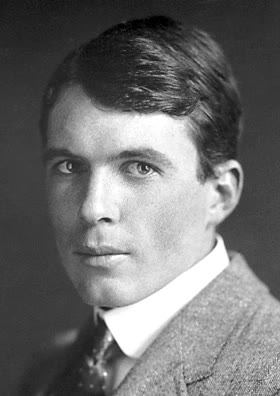
\includegraphics[width=\linewidth]{images/book4/bragg-wl.jpg}\par
{\footnotesize W. L. Bragg.}
\end{minipage}
\end{history}

\section{Exercícios}

\begin{exercise}[$\star$]\label{exo:b3:x-ray-diffraction:1}
% ledger: lat:NaCl
Para \ce{NaCl} ($a = \qty{564.06}{pm}$), calcule $d_{111}$, $d_{200}$ e $d_{220}$.
\end{exercise}

\begin{exercise}[$\star$]\label{exo:b3:x-ray-diffraction:2}
% ledger: lat:Cu, xray:CuKa1
O cobre é cúbico de faces centradas, com $a = \qty{361.50}{pm}$. Com Cu K$\alpha_1$ ($\lambda = \qty{154.06}{pm}$),
calcule $2\theta$ de suas duas primeiras reflexões, depois de nomeá-las.
\end{exercise}

\begin{exercise}[$\star$]\label{exo:b3:x-ray-diffraction:3}
Quais das reflexões 100, 110, 111, 200, 210, 211, 220 estão presentes para uma
rede cúbica P, I e F?
\end{exercise}

\begin{exercise}[$\star$]\label{exo:b3:x-ray-diffraction:4}
Dê a base recíproca de uma rede retangular bidimensional de lados
$a$ e $b$, e desenhe os primeiros nós recíprocos.
\end{exercise}

\begin{exercise}[$\star\star$]\label{exo:b3:x-ray-diffraction:5}
% ledger: lat:W
Um metal dá linhas em $2\theta = 40.27$, 58.26, 73.20, 87.01 e \ang{100.66} com Cu
K$\alpha_1$. Indexe o difratograma e encontre o tipo de rede e $a$.
\end{exercise}

\begin{exercise}[$\star\star$]\label{exo:b3:x-ray-diffraction:6}
% ledger: lat:KCl
Um cristal de \ce{KCl} ($a = \qty{629.29}{pm}$) tem densidade medida de
\qty{1.99}{g/cm^3} (dados do exercício). Encontre $Z$.
\end{exercise}

\begin{exercise}[$\star\star$]\label{exo:b3:x-ray-diffraction:7}
A linha (200) de um nanopó de \ce{NaCl} ($2\theta = \ang{31.70}$) tem \ang{0.40} de largura,
sem nenhuma contribuição do instrumento. Estime o tamanho dos cristalitos.
\end{exercise}

\begin{exercise}[$\star\star$]\label{exo:b3:x-ray-diffraction:8}
\ce{CsCl} tem \ce{Cs+} em $(0,0,0)$ e \ce{Cl-} em $(\frac12,\frac12,\frac12)$ em uma célula P. Com $f
\approx$ o número de elétrons, calcule $F_{100}$ e $F_{110}$ e a razão de suas
intensidades (apenas o \omterm{def:b3:x-ray-diffraction:structure-factor}{fator de estrutura}). Por que \ce{CsCl} não é de corpo centrado?
\end{exercise}

\begin{exercise}[$\star\star$]\label{exo:b3:x-ray-diffraction:9}
Mostre que uma rede de bases centradas C (nó extra em $(\frac12,\frac12,0)$) torna ausentes
as reflexões com $h + k$ ímpar.
\end{exercise}

\begin{exercise}[$\star\star\star$]\label{exo:b3:x-ray-diffraction:10}
Explique por que a descoberta, nos anos 1980, de ligas cujos difratogramas
mostram manchas nítidas com simetria de ordem dez não contradisse a restrição
cristalográfica, e o que ela mudou na definição de cristal.
\end{exercise}

\begin{exercise}[$\star\star\star$]\label{exo:b3:x-ray-diffraction:11}
Mostre que em \textit{P}$2_1/c$ o \omterm{def:b3:x-ray-diffraction:space-group}{plano de deslizamento} torna ausentes as reflexões $h0l$ com $l$
ímpar.
\end{exercise}

\begin{exercise}[$\star\star\star$]\label{exo:b3:x-ray-diffraction:12}
Um enantiômero puro nunca pode cristalizar em um \omterm{def:b3:x-ray-diffraction:space-group}{grupo espacial} que contenha um
\omterm{def:b3:point-groups:inversion}{centro de inversão}, um espelho ou um \omterm{def:b3:x-ray-diffraction:space-group}{plano de deslizamento}. Por quê? A que tipo de
\omterm{def:b3:x-ray-diffraction:space-group}{grupos espaciais} ele está restrito, e o que a lei de Friedel implica para a
determinação de sua configuração absoluta?
\end{exercise}

% keep the heading with its problem box, which fills a page by itself
\clearpage
\enlargethispage{3\baselineskip}
\section{Problema: Qual pó branco?}

\begin{problem}[{Problema de fim de semana --- o difratograma de pó de um sal cúbico
desconhecido: distâncias, indexação, o parâmetro de rede e a identidade do sal,
e o tamanho de seus cristalitos}]
\label{pb:b3:x-ray-diffraction:1}
% ledger: xray:CuKa1, lat:NaCl, lat:KCl, lat:KBr
Um pó cristalino branco desconhecido, que se sabe ser \ce{NaCl}, \ce{KCl} ou \ce{KBr},
dá com a radiação Cu K$\alpha_1$ ($\lambda = \qty{154.059}{pm}$) as linhas (dados do
problema, calculados para este exercício):
\begin{center}\small
\begin{tabular}{lcccccc}
\hline
$2\theta$ / grau & 28.342 & 40.512 & 50.178 & 58.632 & 66.380 & 73.692 \\
intensidade relativa & 100 & 92 & 38 & 20 & 61 & 49 \\ \hline
\end{tabular}
\end{center}
Nenhuma outra linha aparece entre 20 e \ang{75}. Parâmetros de rede de referência:
\ce{NaCl} \qty{564.06}{pm}, \ce{KCl} \qty{629.29}{pm}, \ce{KBr} \qty{658.47}{pm}. Massas molares:
K 39.1, Na 23.0, Cl 35.5, Br \qty{79.9}{g/mol}.

\medskip\noindent\textbf{Parte I --- Distâncias.}
\begin{enumerate}
  \item Calcule $\theta$ e $d$ para a primeira linha.
  \item Calcule $d$ para todas as linhas.
  \item Calcule as razões $\sin^2\theta/\sin^2\theta_1$.
  \item Que série de inteiros você encontra?
  \item O difratograma poderia ser o de uma rede cúbica primitiva? Com que $a$?
  \item Para uma rede cúbica primitiva, que inteiro $N$ nunca pode ocorrer? O
        difratograma permite, até aqui, distinguir as duas interpretações?
\end{enumerate}

\medskip\noindent\textbf{Parte II --- A rede real.}
\begin{enumerate}[resume]
  \item Os três candidatos são redes F. Indexe as linhas com a série F.
  \item Deduza $a$ a partir da primeira linha.
  \item Qual candidato se ajusta?
  \item Para esse sal, por que as reflexões todas ímpares (111), (311) estão ausentes?
  \item O \ce{NaCl} mostraria (111)? E o \ce{KBr}?
  \item Explique por que a interpretação primitiva da Parte I é uma armadilha.
\end{enumerate}

\medskip\noindent\textbf{Parte III --- Densidade e conteúdo.}
\begin{enumerate}[resume]
  \item Quantas unidades de fórmula a célula contém?
  \item Calcule a densidade a partir da célula.
  \item Dê o número de coordenação de cada íon.
  \item Calcule a menor distância K--Cl.
  \item Que reflexão apareceria primeiro acima de \ang{75}?
  \item Por que as intensidades são menos úteis que as posições para identificar uma fase?
\end{enumerate}

\medskip\noindent\textbf{Parte IV --- Refinamento e tamanho dos cristalitos.}
\begin{enumerate}[resume]
  \item Por que o parâmetro de rede é mais bem calculado a partir de uma linha de ângulo alto?
  \item Calcule $a$ a partir da linha (420).
  \item A linha (420) tem \ang{0.25} de largura em $2\theta$ (largura instrumental
        desprezível). Estime o tamanho dos cristalitos.
  \item Um tamanho de cristalito de \qty{1}{\micro m} alargaria a linha de modo mensurável?
  \item Enuncie o resultado: o parâmetro de rede refinado a partir da linha (420) e
        a identidade do pó.
\end{enumerate}
\end{problem}
